%Root main.tex
%---------------------------------------------------------------------------
%付録A　付録
%---------------------------------------------------------------------------
% --- プリアンブルに追加してください ---
% \usepackage{float}
% \usepackage{listings}
% ----------------------------------

%Root main.tex
%---------------------------------------------------------------------------
%付録A　付録
%---------------------------------------------------------------------------

\chapter{PSIMを用いたシミュレーション}
\thispagestyle{fancy}
\label{chap:MATLAB}
本研究ではプラス株式会社のPSIMを用いてシミュレーションを行った．PSIMではパワーエレクトロニクスの解析，制御系回路設計，インバータ，モータドライブの研究に対して有効なシミュレーション環境が提供されている．シミュレーションにおける制御部分は，Cブロックに書き込むことによって実装することができる．表\ref{tabA.1}にPSIMの実行環境を示す．

\begin{table}[H]
    \centering
    \caption{PSIMの実行環境}
    \label{tabA.1}
    \small
    \begin{tabular}{c|c} \hline \hline
        実行OS    &   ソフトバージョン    \\ \hline
        Windows11    & PSIM 2025a   \\ \hline
    \end{tabular}
\end{table}

表\ref{tabA.2}に本研究で使用したPSIMの実行ファイル名，保存場所を示す．

\begin{table}[H]
    \centering
    \caption{ファイル情報}
    \label{tabA.2}
    \small
    \begin{tabular}{l|l} \hline \hline
        実行ファイル名  & TMEIC\_LC\_main\_疑似dq.psimsch \\
                        & CCBPF.psimsch \\ \hline
        保存場所        & 「box」/「0-横山研究室資料共有フォルダ」/「ミーティング資料」/「系統」\\
                        & /「2025年度」/「yamazaki」/「卒論psimファイル」 \\ \hline
    \end{tabular}
\end{table}

本検証で使用したシミュレーションファイルは，TMEIC\_LC\_main\_疑似dq.psimschとCCBPF.psimschのみである．

\section{疑似dq変換のシミュレーション}
図\ref{FigA.1}に定常運転時の連携リアクトルなし三相系統連系システムを主回路図を示す．

\begin{figure}[H]
    \centering
    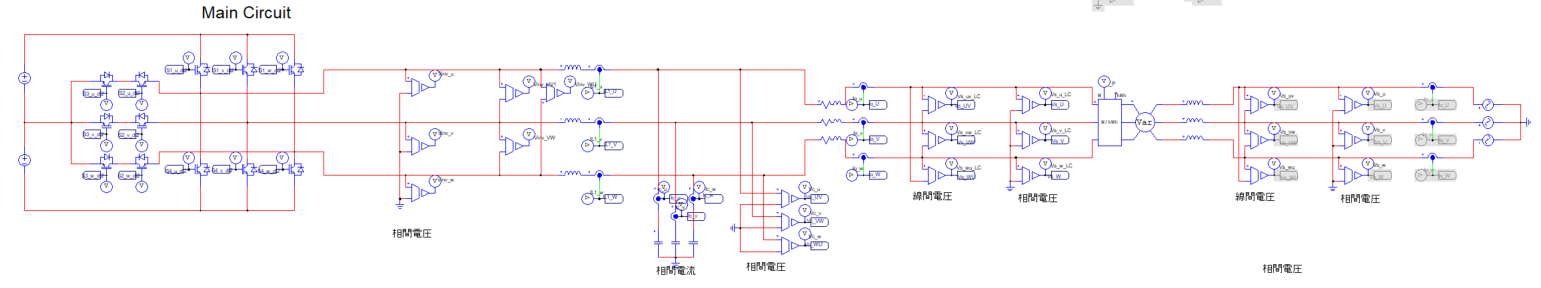
\includegraphics[width=140mm]{image/2025/1.png}
    \caption{定常運転時の連携リアクトルなし三相系統連系システムを主回路図}
    \label{FigA.1}
\end{figure}

図\ref{FigA.1}について，系統システムの制御に用いる状態変数の電流，電圧はそれぞれセンサから値を取得，もしくは数値計算によって導出する．
図\ref{FigA.2}に制御と状態変数のホールドを行うモジュールを示す．

\begin{figure}[H]
    \centering
    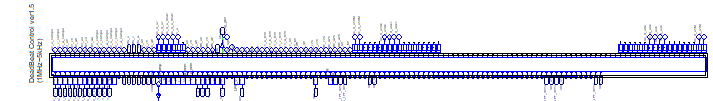
\includegraphics[width=140mm]{image/2025/2.png}
    \caption{制御と状態変数のホールドを行うモジュール}
    \label{FigA.2}
\end{figure}

図\ref{FigA.2}のCブロックでは，電流指令値の生成，デッドビート制御，パルス指令値の生成などを行なっている．
図\ref{FigA.4}に三角波比較のモジュールを示す．

\begin{figure}[H]
    \centering
    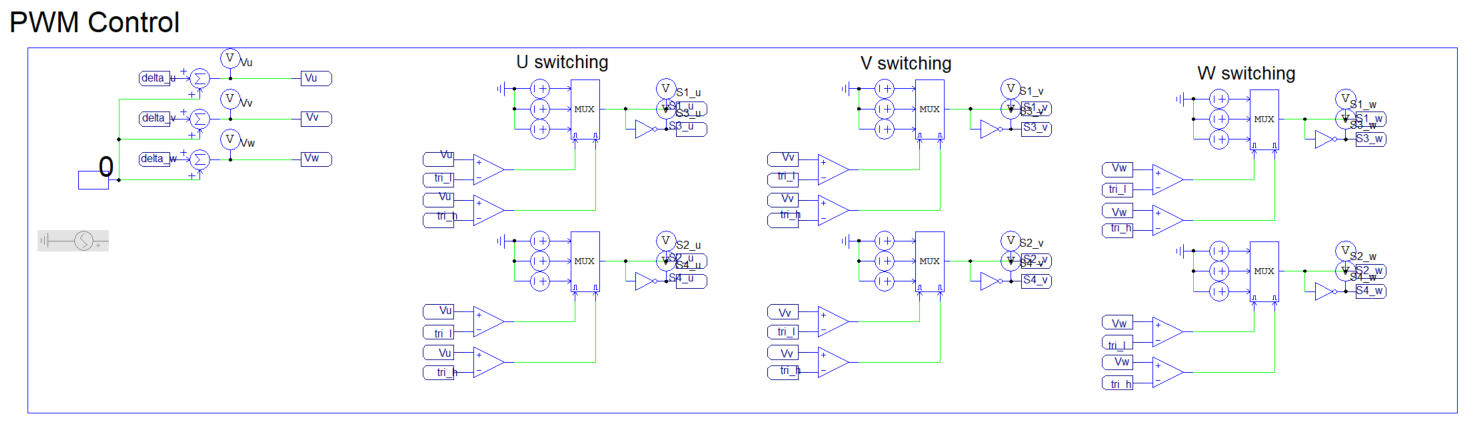
\includegraphics[width=80mm]{image/2025/3.png}
    \caption{三角波比較のモジュール}
    \label{FigA.4}
\end{figure}

図\ref{FigA.4}では，Cブロックで生成したU相のパルス$u_{u}$，V相のパルス指令値$u_{v}$，W相のパルス指令値$u_{w}$について三角波比較を行い，インバータのゲート信号を生成する．図\ref{FigA.5}にデッドタイム生成モジュールを示す．

\begin{figure}[H]
    \centering
    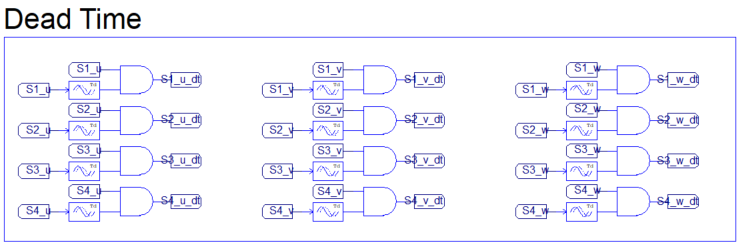
\includegraphics[width=140mm]{image/2025/4.png}
    \caption{デッドタイム生成モジュール}
    \label{FigA.5}
\end{figure}

図\ref{FigA.5}では，三角波比較により生成したゲート信号に対してデッドタイム処理を行うことで，インバータの各レグのアームが同時にONになるのを防ぐ処理を行う．

図\ref{FigA.6}にパラメータを示す．

\begin{figure}[H]
    \centering
    
\includegraphics[width=60mm]{image/appendixA/FigA.6.png}
    \caption{パラメータファイル}
    \label{FigA.6}
\end{figure}

図\ref{FigA.6}は，回路のパラメータやキャリア周期，サンプリング周期などを書き込むファイルである．

図\ref{FigA.7}に疑似dq変換の3サンプリング取得モジュールを示す．
\begin{figure}[H]
    \centering
    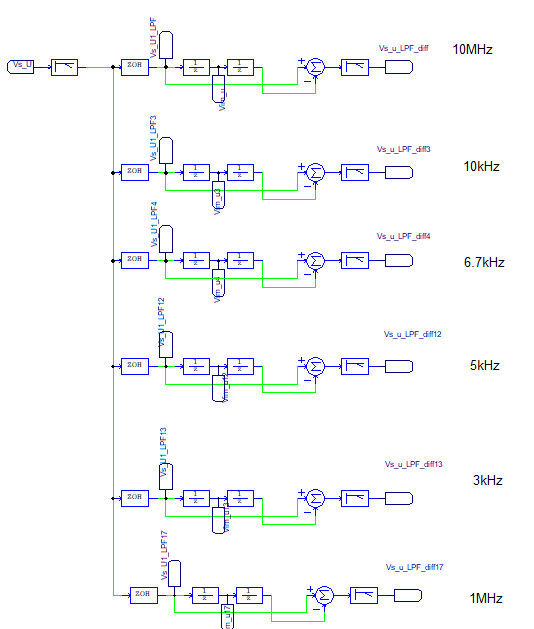
\includegraphics[width=80mm]{image/2025/5.png}
    \caption{疑似dq変換の3サンプリング取得モジュール}
    \label{FigA.7}
\end{figure}

図\ref{FigA.7}では，系統電圧をセンサにより取得し，零次ホールドによりサンプリング周波数でホールドする．
ホールドした後のデータを1サンプル目とする．次に単位遅れブロックにより1サンプル遅らせることで2サンプル目を生成する．
2サンプル目を虚軸のサンプリングデータとする．
さらにもう一度単位遅れブロックにより1サンプル遅らせることで3サンプル目を生成する．
このようにして，3サンプリング分の系統電圧のデータを取得する．
1サンプル目と3サンプル目のデータの差分をとる．

\section{複素係数フィルタのシミュレーション}
図\ref{FigA.8}に複素係数フィルタモジュールを示す．

\begin{figure}[H]
    \centering
    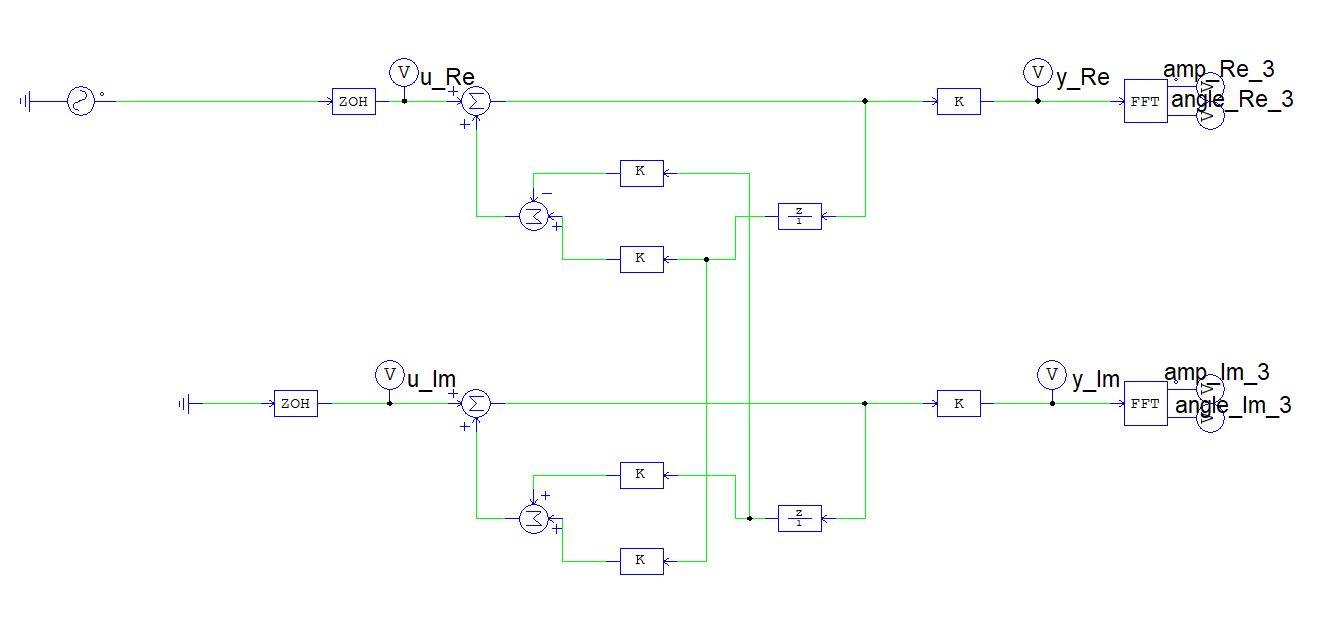
\includegraphics[width=140mm]{image/2025/6.png}
    \caption{複素係数フィルタモジュール}
    \label{FigA.8}
\end{figure}

図\ref{FigA.8}では，上部を実数部，下部を虚数部としている．入力電圧は実部のみに入力信号を入力している．
複素係数フィルタの出力は，上部に実部の出力を，下部に虚数部の出力を出力している．
PSIMでは虚数演算ができないため，実部と虚部を分けて計算する必要がある．

\section{DC-MSSRDB\_Control}
連携リアクトルなし三相系統連系システムにおけるプログラムリストをソースコード\ref{lisA.1}に示す．

\lstinputlisting[
    language=C,
    caption={DC-MSSRDB\_Control},
    label={lisA.1},
    basicstyle=\small\ttfamily,
    frame=single,
    breaklines=true
]{image/2025/lisA.1.c}